\documentclass[aspectratio=169]{beamer}

\usetheme{Boadilla}
\usefonttheme{professionalfonts}
\usefonttheme{structuresmallcapsserif}

\usepackage{amsmath, latexsym, amsfonts, amssymb, amsthm}
\newtheorem{remark}[theorem]{Remark}
\newtheorem{observation}[theorem]{Observation}

\usepackage[T1]{fontenc}
\usepackage{garamondx}
\usepackage[garamondx,cmbraces]{newtxmath}
\usepackage{listings}

\setbeamertemplate{section page}
{
    \begin{centering}
    \usebeamerfont{section title}\usebeamercolor[fg]{section name}\sectionname~\MakeUppercase{\romannumeral\insertsectionnumber}\\
    \begin{beamercolorbox}[sep=12pt,center]{part title}
    \usebeamerfont{section title}\insertsection\par
    \end{beamercolorbox}
    \end{centering}
}
\defbeamertemplate{section in toc}{sections numbered roman}{%
  \leavevmode%
  \MakeUppercase{\romannumeral\inserttocsectionnumber}.\ %
  \inserttocsection\par}
\setbeamertemplate{section in toc}[sections numbered roman]

\title[DKRV14 and DMS14]{Unit volume Liouville measure on the sphere with $(\gamma,\gamma,\gamma)$-insertions: the link between two constructions}
\author[Yichao Huang]{Yichao Huang$^{[ENS]}$, joint with Juhan Aru$^{[ETH]}$, Xin Sun$^{[MIT]}$}
\date[IH\'ES, 17 May 2016]{}

\begin{document}
\AtBeginSection{\frame{\sectionpage}}

\begin{frame}
\titlepage
\end{frame}

\begin{frame}
\frametitle{Introduction}
\framesubtitle{Motivation: Liouville Quantum Gravity}
Two constructions of random measures on the sphere by David$^\circ$, Duplantier$^\bullet$, Kupiainen$^\circ$, Miller$^\bullet$, Rhodes$^\circ$, Sheffield$^\bullet$, Vargas$^\circ$.\\
$\circ=[DKRV14]$, $\bullet=[DMS14]$.\\
Goal: find a link between these two constructions.\\
~\\
Warning: due to time constraints, we will make some inaccurate descriptions on purpose.

\end{frame}

\begin{frame}
\frametitle{Outline}
\tableofcontents
\end{frame}


\section{Gaussian Free Field}

\begin{frame}
\frametitle{Whole plane GFF}
\framesubtitle{as a $\log$-correlated Gaussian field}
\begin{definition}
A whole plane GFF (under $d\mathbb{P}$) is a Gaussian field $(X(z))_{z\in\mathbb{R}^2}$ with correlation function
$$\mathbb{E}[X(x)X(y)]=-\ln|x-y|.$$
\end{definition}
A whole plane GFF is defined \emph{modulo a constant}. One can fix this by first considering\\
-- a whole plane GFF \only<1>{such that ``$X(0)=0$''}\only<2>{such that $\int_{A}X(z)dg(z)=0$};\\
-- add to it an independent (possibly random) constant component $c$.
\end{frame}

\begin{frame}
\frametitle{Orthogonal decomposition of the whole plane GFF}
\framesubtitle{feat. Brownian motions}
\begin{theorem}[Circle-average decomposition]
Let $X(z)$ be a whole-plane GFF (on $\mathbb{R}^2$). We can decompose $X$ into two independant parts:\\
-- $R(z)=R(|z|)$, which is the average of $X$ on circles $\partial B(0,r)$;\\
-- $N(z)$, and is of average $0$ on circles $\partial B(0,r)$. This part can be defined abstractly.\\
We have $X(z)=R(z)\oplus N(z)$.\\
\end{theorem}
Moreover, $R(e^{-t})$ is a Brownian motion!\\
Example: if we choose to study the whole plane GFF such that ($\partial\mathbb{D}=\partial B(0,1)$ the unit circle)
$$\int_{\partial{\mathbb{D}}}X(z)d\lambda_{\partial}(z)=0,$$
then $R(e^{-t})$ is a standard Brownian motion on $\mathbb{R}$ with $R(0)=0$.
\end{frame}


\section{Insertions: classical and quantum}

\begin{frame}
\frametitle{Classical insertions}
\framesubtitle{a.k.a. conical singularities}
\begin{definition}
A (conformal) metric $ds^2$ on a Riemann surface $S$ has a \emph{conical singularity} of order $\beta$ ($\beta$ a real number $>-1$) at a point $p\in S$ if in some neighbourhood of $p$:
$$ds^2=e^{2u}|dz|^2$$
where $z$ is a coordinate of $S$ defined in this neighbourhood and $u$ is a function such that
$$u(z)-\beta\log|z-z(p)|$$
is continuous at $p$.
\end{definition}
\end{frame}

\begin{frame}
\frametitle{Classical insertions}
\framesubtitle{a.k.a. conical singularities}
\begin{block}{Sphere with two antipodal singularities (by Troyanov)}
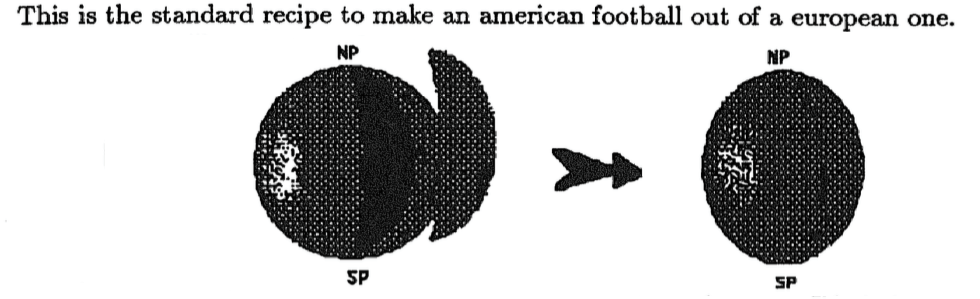
\includegraphics[width=\textwidth]{Football.png}
\end{block}
\end{frame}

\begin{frame}
\frametitle{Quantum insertions}
\framesubtitle{a.k.a. vertex operators}
We shift the measure by the exponential term $e^{\alpha X(z_i)}$ to create an insertion at point $z_i$.
\begin{theorem}[Girsanov theorem]
The law of a gaussian field $X$ under the measure $d\mathbb{P}$ is the same as the law of $X-\alpha\mathbb{E}[X(\cdot)X(z_i)]$ under the measure $e^{\alpha X(z_i)}d\mathbb{P}$.
\end{theorem}
For a whole plane GFF, $\mathbb{E}[X(\cdot)X(z_i)]=-\ln|\cdot-z_i|$: the nature of singularities is conical.
\end{frame}

\begin{frame}
\frametitle{The DKRV definition}
\framesubtitle{of the unit volume Liouville measure}
\begin{definition}[Unit volume Liouville measure]
Let $g$ be a metric on the sphere. Let $X_g$ be a whole plane GFF such that $\int_{\mathbb{R}^2}X_g(z)dg=0$.
Consider
$$X_L=X_g(z)+\frac{Q}{2}\ln g(z)+\sum_i\alpha_i\ln|z-z_i|$$
and let $Z_\gamma(\mathbb{R}^2)=\int_{\mathbb{R}^2}e^{\gamma X_L(z)}d\lambda$ the volume form associated with $X_L$.\\
The law of the unit volume Liouville measure is given by
$$\mu(A)=\int_{A}e^{\gamma X_U(z)}d\lambda$$
where $X_U=X_L-\frac{1}{\gamma}\ln Z_\gamma(\mathbb{R}^2)$ under the measure $Z_\gamma(\mathbb{R}^2)^{\frac{2Q-\sum_i\alpha_i}{\gamma}}d\mathbb{P}$.
\end{definition}
\end{frame}

\begin{frame}
\frametitle{Effect of insertions on the radial part}
\framesubtitle{feat. drifted Brownian motions and Bessel process}
\begin{lemma}
If we add $\gamma\log|z-0|$ to the whole plane GFF $X$, its radial part $R(|z|)$ verifies
$$R(e^{-t})=B(t)-\gamma t$$
which is a Brownian motion with drift (we don't require $B(0)=0$ yet).
\end{lemma}
With two $\gamma$-insertions at $0$ and $\infty$, the radial part is a \emph{``two-sided drifted Brownian motion''}.\\
How to define such an object? We must consider an equivalence class (modulo lateral shifts).\\
We can describe such object by Bessel excursion.
\end{frame}

\begin{frame}
\frametitle{The DMS random measure}
\framesubtitle{with two $\gamma$-insertions at $0$ and $\infty$}
\begin{lemma}
Let $\delta=4-8/\gamma^2$ and $\nu^{BES}_\delta$ the Bessel excursion measure of dimension $\delta$.\\
We sample the radial part $R$ of $X_U$ in the following way:\\
1. Sample a Bessel excursion $\mathfrak{e}$ w.r.t. $\nu^{BES}_\delta$;\\
2. Reparametrizing $\frac{1}{\gamma}\log\mathfrak{e}$ to have unit quadratic variation.\\
Adding the orthogonal $N$ part, we get the law of $X_U$ under $d\mathbb{P}$.
\end{lemma}
The law of the maximum of this Bessel process is linked to the reweighting coefficient in the DKRV formulation.
\end{frame}

\begin{frame}
\frametitle{The wrong theorem}
\begin{theorem}[Naive version]
Consider the DKRV measure with two $\gamma$-insertions at $0$ and $\infty$.\\
Then we get the DMS random measure.
\end{theorem}
Problem: Seiberg bound\dots
\end{frame}


\section{Theorem and consequences}

\begin{frame}
\frametitle{Main theorem of [AHS15]}
\framesubtitle{From DMS14 to DKRV14}
For better comprehension, we state the theorem in plain words.
\begin{theorem}[AHS15]
Take the sphere, or the whole plane.\\
1. Consider the DMS measure with two $\gamma$-insertions at $0$ and $\infty$;\\
2. Pick a third point $z$ w.r.t. this measure;\\
3. Use a conformal map that shifts $(0,z,\infty)$ to $(0,1,\infty)$;\\
4. Push-forward the DMS measure by this conformal map;\\
5. We get DKRV measure with three $\gamma$-insertions at $0$, $1$ and $\infty$!
\end{theorem}
\end{frame}

\begin{frame}
\frametitle{Consequences}
\framesubtitle{From DKRV14 to DMS14\dots}
\begin{remark}[Consequence I]
1. Take DKRV measure with three $\gamma$-insertions at $0$, $1$ and $\infty$;\\
2. Forget about the point $1$, and pass to the quotient space $\mathcal{Q}$ by lateral shift;\\
3. We get the DMS measure with two $\gamma$-insertions at $0$ and $\infty$.
\end{remark}
\begin{remark}[Consequence II]
1. Take DKRV measure with two $\gamma$-insertions at $0$, $\infty$ and one $\epsilon$-insertion point at $1$;\\
2. Let $\epsilon$ go to $0$;\\
3. We get the DMS measure with two $\gamma$-insertions at $0$ and $\infty$.
\end{remark}
\end{frame}

\begin{frame}
\frametitle{Thanks!}
\begin{block}{Isaac Newton Institute for Mathematical Sciences}
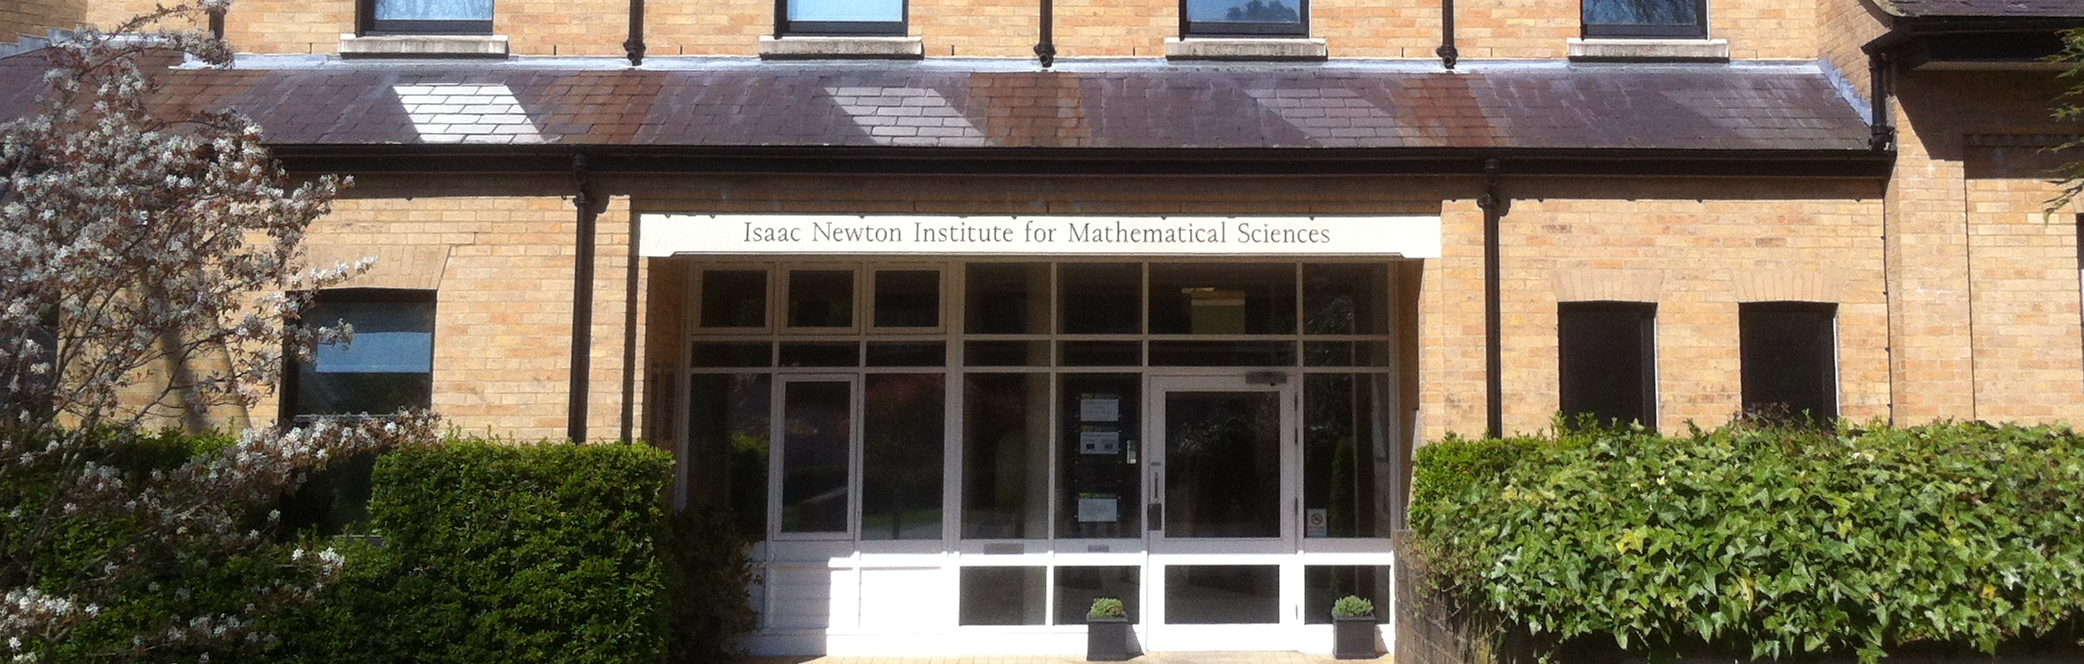
\includegraphics[width=\textwidth]{INI.png}
\end{block}
\end{frame}

\end{document}
